\scanpage{132}
\figure{
\begin{tikzpicture}[scale=.55]
\draw (0,0)--(-.9,-1.3).. controls (-.3,-.8) and (.3,-.2) ..(-.1,-1.3)--(-.65,-2.3);
\draw (-.65,-2.3)--(.45,-.6)--(.05,-2.15);
\draw[gray] (.85,-.55)--(.35,-2.4);
\draw[gray] (.2,-2.2)--(.35,-2.55);
\end{tikzpicture}}
\figure{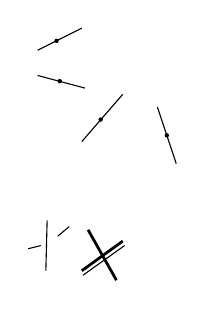
\begin{tikzpicture}[scale=.8]
\draw (0,2)--(.7,2.35);\fill (.3,2.15) circle(.035);
\draw (0,1.6)--(.75,1.4);\fill (.35,1.51) circle(.035);
\draw (.7,.55)--(1.35,1.3);\fill (1, .9) circle(.035);
\draw (1.9,1.1)--(2.2,.2);\fill (2.05,.65) circle(.035);
\draw (-.15,-1.15)--(.05,-1.1);\draw (.15,-.7)--(.13,-1.5);\draw (.32,-.95)--(.5,-.8);
\draw[line width=1pt] (.8,-.85)--(1.25,-1.65);\draw[line width=1pt](.7,-1.5)--(1.35,-1.03);\draw(.72,-1.57)--(1.38,-1.1);
\end{tikzpicture}}
\rotatebox{90}{$\begin{array}{ll}
\deleted{\unsure{k[x^i|k[x}}&\unsure{x^2|x^3}-y^2\\
&k[y]\qquad\unsure{12,13|p^2,p^3}\\
&k[x,y]/xy
\end{array}$}

\rotatebox{180}{\begin{tabular}{c}
INSTITUT\\
DES HAUTES ÉTUDES SCIENTIFIQUES\\
\rule{1cm}{.4pt}
\end{tabular}}
\margin{131}
